\begin{figure}[thb]
  \centering
  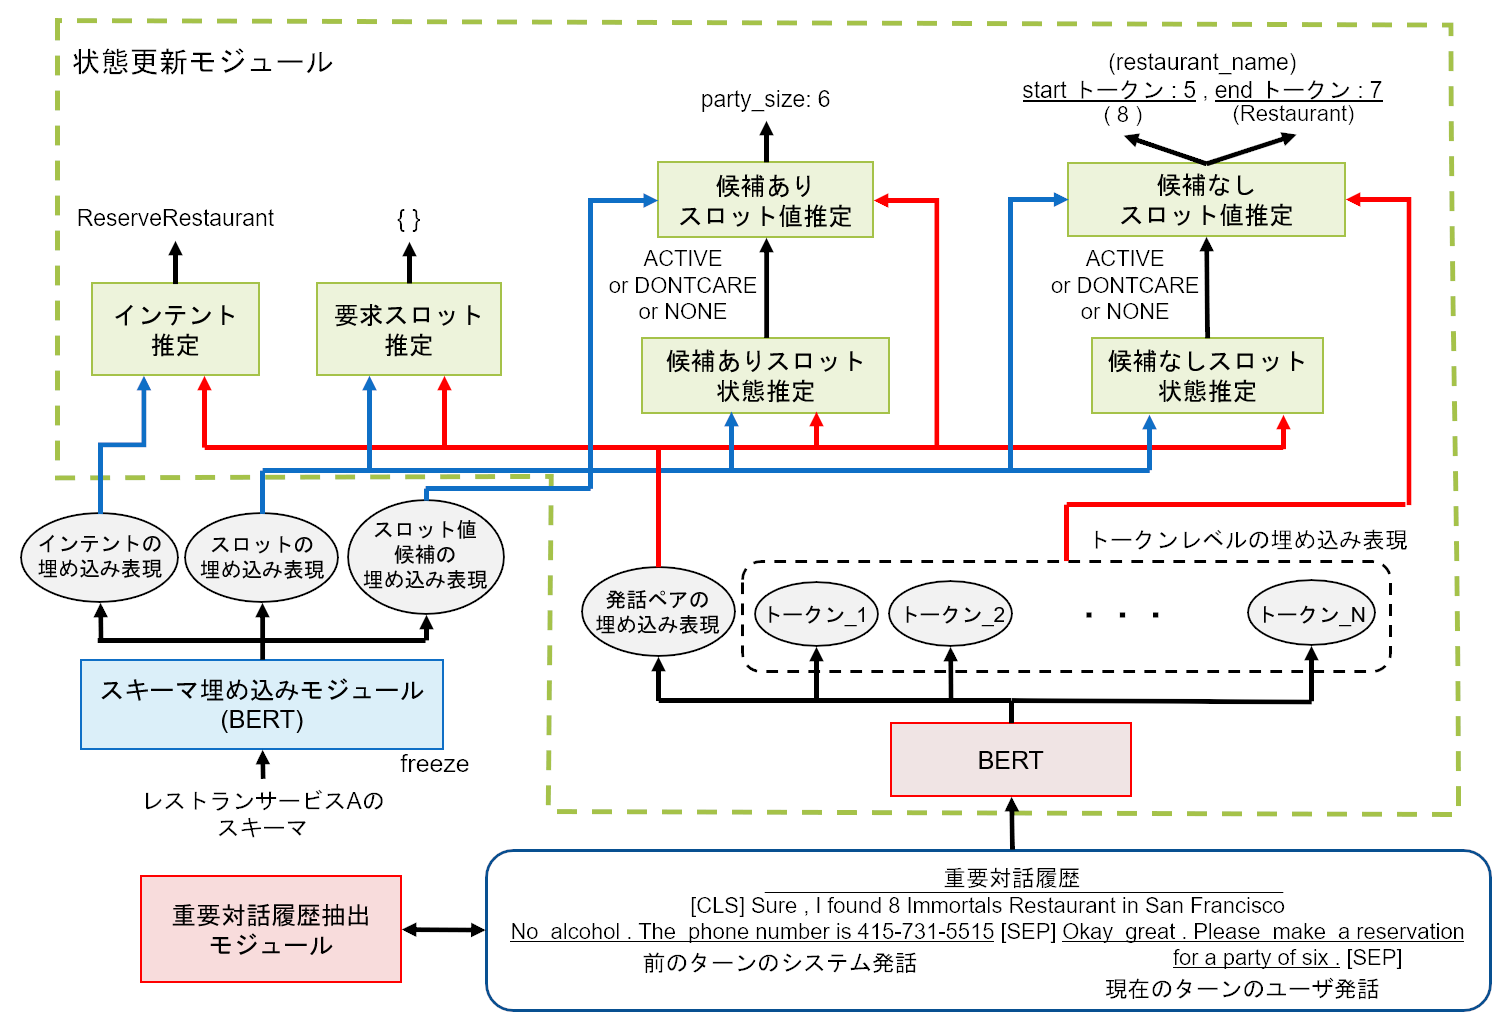
\includegraphics[width=15cm]{chapter4/teian.eps}
  \caption{重要対話履歴抽出モジュールを加えた提案モデル}
  \label{fig:teian}
\end{figure}

\begin{table}[thb]
  \centering
  \caption{SGDデータセットにある対話例の一部}
  \label{tab:taiwarei}
  \begin{tabular}{|p{55mm}|l|}\hline
    \multicolumn{1}{|c|}{
    \begin{tabular}{c}
      発話文\\(U:ユーザ,S:システム)
    \end{tabular}
    } 
    & \multicolumn{1}{|c|}{
      \begin{tabular}{c}
      対話状態(ユーザのターン時)\\or\\対話行為(システムのターン時)
    \end{tabular}
     } \\ \hline \hline
    \begin{tabular}{l}
      U1: Can you pull up a list of \\places to eat?
    \end{tabular} &
    \begin{tabular}{l}
      \{インテント:FindRestaurant, 要求スロット:[ ],\\ スロット値:\{\} \}
    \end{tabular} \\ \hline
    \begin{tabular}{l}
      S1: Sure, what city should I \\search? And what kind of food \\would you like?
    \end{tabular} &
    \begin{tabular}{l}
    \{ REQUEST(city, [ ]), REQUEST(cuisine, [ ]) \}
    \end{tabular} \\ \hline
    \begin{tabular}{l}
      U2: Search San Francisco for \\Asian Fusion food
    \end{tabular} & 
    \begin{tabular}{l}
      \{インテント:FindRestaurant, 要求スロット:[ ],\\スロット値:\{ city: San Fracisco, \\cuisine: Asian Fusion \} \}
    \end{tabular} \\ \hline
    \begin{tabular}{l}
      S2: Sure, I found 8 Immortals \\Restaurant in San Francisco 
    \end{tabular}& 
    \begin{tabular}{l}
      \{ OFFER(restaurant\_name, 8 Immortals \\Restaurant), OFFER(city, San Francisco) \}
    \end{tabular} \\ \hline
    \begin{tabular}{l}
      U3: Is there live music?
    \end{tabular} & 
    \begin{tabular}{l}
      \{インテント:FindRestaurant, 要求スロット:[ \\has\_live\_music ], スロット値:\{ city: San Fracisco, \\cuisine: Asian Fusion \} \}
    \end{tabular} \\ \hline
    \begin{tabular}{l}
      S3: Unfortunately no.
    \end{tabular} & 
    \begin{tabular}{l}
      \{ INFORM(has\_live\_music, False) \}
    \end{tabular} \\ \hline
    \begin{tabular}{l}
      U4: Do they serve alcohol? \\And what's their phone \\number?
    \end{tabular} & 
    \begin{tabular}{l}
      \{インテント:FindRestaurant, 要求スロット:[ \\phone\_number, serves\_alcohol ], スロット値:\{ city: \\San Fracisco, cuisine: Asian Fusion \} \}
    \end{tabular} \\ \hline
    \begin{tabular}{l}
      S4: No alcohol. The phone \\number is 415-731-5515 
    \end{tabular}& 
    \begin{tabular}{l}
      \{ INFORM(serves\_alocohol, False), \\INFORM(phone\_number, 415-731-5515) \}
    \end{tabular} \\ \hline
    \begin{tabular}{l}
      U5: Okay great. Please make \\a reservation for a party of six.
    \end{tabular} & 
    \begin{tabular}{l}
      \{ インテント:ReserveRestaurant, 要求スロット:\\
      \verb|[ ]|, スロット値:\{ city: San Fracisco, cuisine: \\Asian Fusion, party\_size: 6, restaurant\_name: \\8 Immortals Restaurant \} \}
    \end{tabular} \\ \hline
  \end{tabular}
\end{table}
  
ベースラインモデルが過去の対話の流れを捉えられるようにするために,過去の対話履歴を用いる.深層学習による対話状態追跡で対話履歴を用いる場合,直近の数発話を履歴として入力に用いる\cite{trade,mrc}.しかし,直近の数発話では計算量の観点から多くの発話を入力するのは困難である.そこで,本研究では対話状態追跡に特に重要な発話をモデルへ入力するために,対話行為タグに基づく履歴抽出を提案する.この手法により,履歴として用いる発話を対話状態の推定に必要な情報を持った発話のみにする.そのような発話を重要対話履歴とする.
\par

図\ref{fig:teian}に示す提案モデルでは,ベースラインモデルの入力文を作成する箇所に重要対話履歴を抽出する重要対話履歴抽出モジュールを加えた.このモジュールは,入力文中にある前のターンのシステム発話が特定の対話行為タグを持つ場合に,その発話を保持する.既に発話を保持している場合は,新しい発話に更新する.そして,元々保持されていた発話を重要対話履歴として入力に加える.入力は,重要対話履歴,前のターンのシステム発話,現在のターンのユーザ発話の 3 発話となる.
\par
図 \ref{fig:teian} では,例として表\ref{tab:taiwarei}の対話行為タグ“OFFER”を持つ発話を抽出している.入力に加えられた重要対話履歴には,レストラン名を示す“restaurant\_name”のスロット値となる“8 Immortals Restaurant”が含まれる.入力文にスロット値となる文字列が含まれるため,スロット値として抜き出すことが可能になる.直近の数発話を対話履歴として用いる従来手法の場合は,直近の 6 発話を入力に加える必要があるが,提案手法では 3 発話で推定が行える.また,図\ref{fig:teian}では6ターン前の発話を抽出したが,提案手法はさらに前の発話を抽出することも可能である.ゆえに,提案手法は計算量の削減と同時に性能の向上が期待できる.